\section{FuzzyLogic}
\begin{wrapfigure}{r}{0.4\textwidth}
    \vspace{-1.1cm}
    \begin{center}
      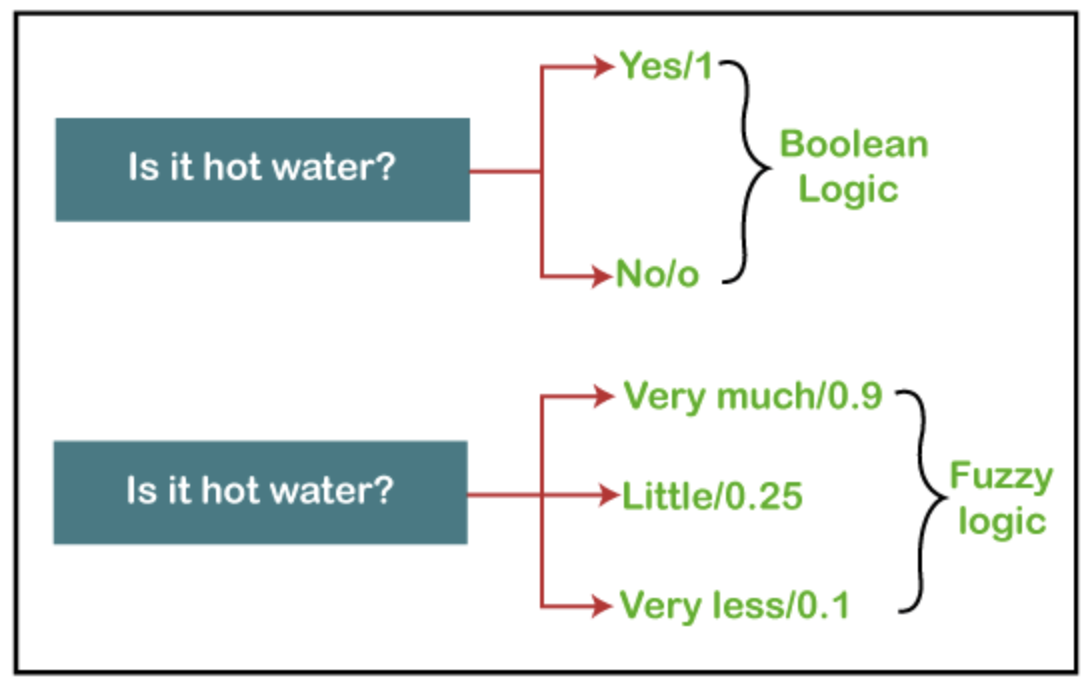
\includegraphics[width=0.4\textwidth]{FuzzyBoolLogic}
    \end{center}
    \vspace{-0.5cm}
    \caption{Vergleich von Fuzzy Logic zu Boolischer Logik \cite{FuzzyLogicTPoint}}
    \label{fig:FuzzyCompare}
    \vspace{-0.5cm}
  \end{wrapfigure}
Fuzzy Logic, erstmals in den 1960er Jahren von Lotfi Zadeh an der University of California entwickelt, stellt einen innovativen Ansatz der Datenverarbeitung dar, der auf Wahrheitsgraden basiert. Im Gegensatz zur herkömmlichen Booleschen Logik, die sich auf binäre Zustände von 1 oder 0 bzw. wahr oder falsch stützt, zeichnet sich die Fuzzy Logic durch ihre Fähigkeit aus, die Vielschichtigkeit von Zwischenzuständen zu berücksichtigen.\cite{FuzzyLogicTechTarget}\\
Das zentrale Merkmal der Fuzzy-Logik besteht darin, unpräzise Argumentationsweisen zu modellieren, die eine bedeutende Rolle in der bemerkenswerten Fähigkeit des Menschen spielen, unter Bedingungen der Ungewissheit und Ungenauigkeit rationale Entscheidungen zu treffen (Siehe Abbildung \ref{fig:FuzzyCompare}). Diese Fähigkeit basiert auf unserem Vermögen, aus einem Wissensbestand, der ungenau, unvollständig oder nicht völlig zuverlässig ist, ungefähre Antworten auf Fragen abzuleiten. Anders als in klassischen logischen Systemen strebt die Fuzzy Logic danach, die Grauzonen zwischen klaren Kategorien zu erfassen und somit eine flexiblere und menschlichere Art der Datenverarbeitung zu ermöglichen. Dieser Ansatz hat Anwendungen in verschiedenen Bereichen gefunden, darunter Steuerungssysteme, künstliche Intelligenz, Entscheidungsfindung und mehr. \cite{LoftiFuzzyLogic}

\subsection{Architektur eines Fuzzy Logic Systems}
Ein Fuzzy Logic Systems kann in vier komponenten unterteilt werden (Siehe Abbildung \ref{fig:FuzzyLogicArchitektur}). Jede dieser Komponenten spielt eine entscheidende Rolle für das gesammte System.  
\begin{center}
    \begin{figure}[h]
     \centering
     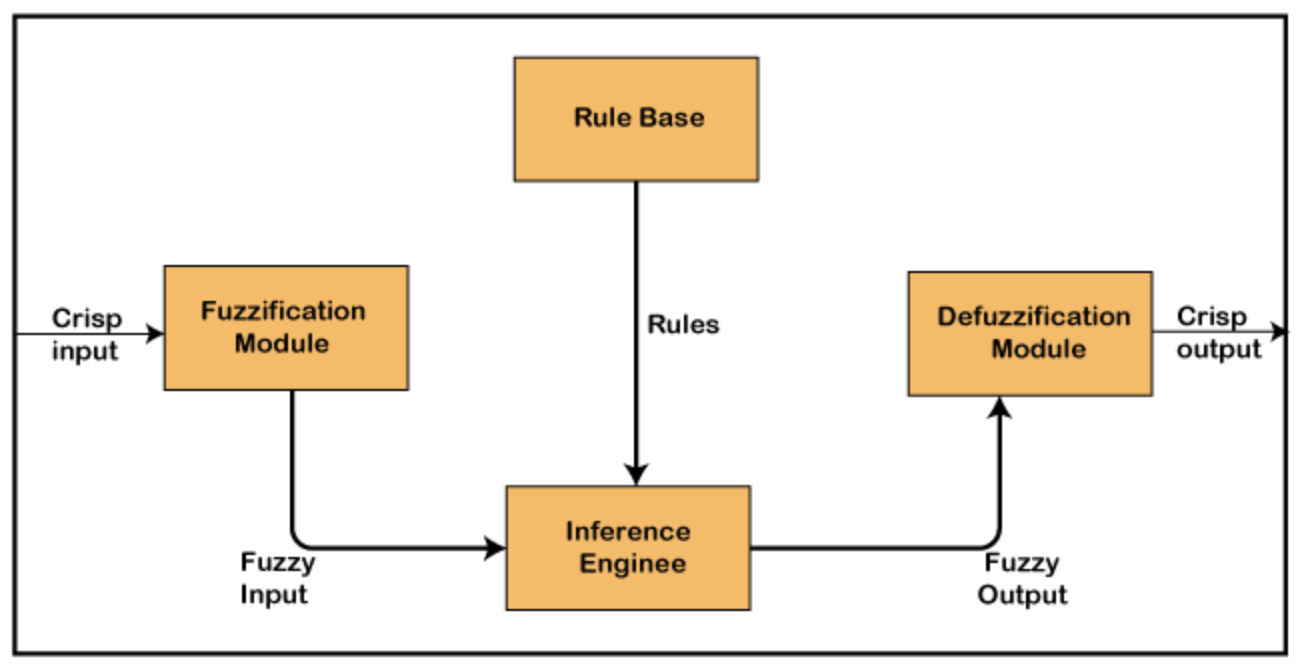
\includegraphics[width=0.6\textwidth]{FuzzyLogicArchitektur}
     \caption{Architektur eines Fuzzy Logic Systems \cite{FuzzyLogicTPoint}}
     \label{fig:FuzzyLogicArchitektur}
    \end{figure}
   \end{center}

